\documentclass[a4paper,11pt]{article}
\usepackage[T1]{fontenc}
\usepackage[utf8]{inputenc}
\usepackage[french]{babel}
\usepackage{lmodern,microtype}
\usepackage[margin=2cm,headheight=14pt,headsep=8mm,footskip=10mm]{geometry}
\usepackage{amsmath,amssymb,graphicx,booktabs,tabularx,array}
\usepackage{xcolor,caption,enumitem,fancyhdr,titlesec}
\usepackage[hidelinks]{hyperref}
\definecolor{polyblue}{HTML}{005479}
\definecolor{amublue}{HTML}{1F63DE}
\definecolor{ink}{HTML}{233447}
\hypersetup{pdftitle={Détection de contours : Sobel, Laplace et Canny},pdfauthor={Omar Benjelloun}}
\graphicspath{{images/}}
\setlength{\parindent}{0pt}
\setlength{\parskip}{4pt}
\setlength{\emergencystretch}{2em}
\renewcommand{\arraystretch}{1.18}
\newcolumntype{Y}{>{\raggedright\arraybackslash}X}
\setlist[itemize]{nosep,leftmargin=1.3em,topsep=3pt}
\captionsetup{font=small,labelfont=bf,skip=5pt}
\titleformat{\section}{\large\bfseries\color{polyblue}}{\thesection}{0.6em}{}
\titleformat{\subsection}{\normalsize\bfseries\color{polyblue}}{\thesubsection}{0.5em}{}
\titlespacing*{\section}{0pt}{11pt}{5pt}
\titlespacing*{\subsection}{0pt}{8pt}{3pt}
\pagestyle{fancy}
\fancyhf{}
\fancyhead[L]{\small Analyse d'images -- TP 3}
\fancyhead[R]{\small Sobel, Laplace et Canny}
\fancyfoot[L]{\small Omar Benjelloun}
\fancyfoot[R]{\small\thepage}
\renewcommand{\headrulewidth}{0.3pt}
\renewcommand{\footrulewidth}{0pt}
\newcommand{\api}[1]{\texttt{#1}}

\begin{document}
\thispagestyle{plain}
\noindent\begin{minipage}[c]{0.58\linewidth}
  
\includegraphics[width=4.9cm]{polytech-marseille.pdf}
\end{minipage}\hfill
\begin{minipage}[c]{0.36\linewidth}\raggedleft
  
\includegraphics[width=3.3cm]{amu.pdf}
\end{minipage}
\vspace{3mm}
\begin{center}
  {\color{polyblue}\LARGE\bfseries Détection de contours}\par
  \vspace{2mm}
  {\large Comparaison de Sobel, Laplace et Canny}\par
  \vspace{3mm}
  Omar Benjelloun\quad--\quad Analyse d'images, Homework 3\par
  {\small Polytech Marseille}
\end{center}
\vspace{1mm}
{\color{amublue}\hrule height 0.6pt}
\vspace{2mm}

\section{Objectif et programme réalisé}
L'objectif est de comparer trois détecteurs sur un lot d'images et de mesurer leur accord avec des contours tracés à la main. Le programme, écrit en \textbf{C++17 avec OpenCV}, propose une interface à curseurs pour choisir l'image, le détecteur et ses paramètres, ainsi qu'un mode par lot qui exporte les cartes de contours et les mesures au format CSV.

La base de Groningen contient \textbf{40 images de $512\times512$ pixels et 40 références}~\cite{groningen}. Dix images servent au réglage, puis les paramètres sont figés pour les trente autres. Les mesures combinent une comparaison pixel à pixel et une comparaison tolérant un décalage d'un pixel.

\section{Détecteurs et paramètres OpenCV}
\subsection{Prétraitement commun}
\api{imread(..., IMREAD\_GRAYSCALE)} charge une image en niveaux de gris 8 bits. Un filtre \api{GaussianBlur} atténue le bruit et les textures : son écart-type $\sigma$ est réglable, avec un noyau de taille $2\lceil3\sigma\rceil+1$ et un bord réfléchi. Dans notre programme, $\sigma=0$ désactive le filtre. Un lissage fort réduit les réponses parasites, mais peut effacer des contours faibles.

\subsection{Sobel : dérivées premières}
Les appels \api{Sobel(..., CV\_32F, 1, 0, k)} et \api{Sobel(..., CV\_32F, 0, 1, k)} approchent les dérivées horizontale et verticale~\cite{sobel}. Leurs réponses sont combinées avec \api{magnitude}, puis seuillées :
\[
  G_x\simeq\frac{\partial I}{\partial x},\qquad
  G_y\simeq\frac{\partial I}{\partial y},\qquad
  E(x,y)=\mathbf{1}\!\left[\sqrt{G_x^2+G_y^2}>T\right].
\]
Le calcul flottant évite la saturation des dérivées. Le seuil $T$ porte sur la réponse brute, sans normalisation par image. Le noyau $k$ modifie le support et l'amplitude de la dérivée. Le seuillage simple peut donner des contours épais.

\subsection{Laplace : dérivées secondes}
\api{Laplacian(..., CV\_32F, k)} calcule $\Delta I=\partial^2 I/\partial x^2+\partial^2 I/\partial y^2$. Nous retenons les pixels pour lesquels $|\Delta I|>T$. Cette version détecte de fortes variations de courbure, mais peut produire des réponses de part et d'autre d'une transition. Elle est sensible au bruit. Il s'agit du \textbf{seuillage du module du Laplacien}, sans recherche des passages par zéro~\cite{laplace}.

\subsection{Canny : amincissement et hystérésis}
\api{Canny(image, contours, bas, haut, k, true)} calcule le gradient, supprime les non-maxima et applique une hystérésis~\cite{canny}. Les réponses fortes sont retenues ; celles entre les deux seuils doivent être reliées à un contour fort. \api{L2gradient=true} utilise la norme euclidienne. Le seuil bas règle les détails candidats, le seuil haut les points de départ fiables. Les contours obtenus sont généralement fins.

\clearpage
\section{Méthode d'évaluation et protocole}
\subsection{Comptages et tolérance géométrique}
Les références de Groningen ont des contours noirs sur fond blanc. Elles sont inversées par un seuillage à 127 pour obtenir des cartes binaires cohérentes avec les sorties du programme. Les mesures utilisent la résolution originale.

On note $D$ le nombre de pixels détectés, $R$ le nombre de pixels de référence et $C$ le nombre de correspondances correctes. Les mesures demandées sont :
\begin{align*}
  FP &= D-C, & FN &= R-C, & Z &= C+FP+FN,\\
  P &= \frac{C}{Z}, & TFP &= \frac{FP}{Z}, & TFN &= \frac{FN}{Z}.
\end{align*}
Ces trois taux somment à 1. Le $TFP$ du sujet diffère du taux de classification $FP/(FP+VN)$. Si les deux cartes sont vides, nous fixons $P=1$ et $TFP=TFN=0$.

En mode exact, les pixels doivent occuper la même position. En mode tolérant, une correspondance est admise dans un voisinage $3\times3$ : au plus un pixel de décalage par axe. Un \textbf{appariement maximum un à un} (Hopcroft--Karp) interdit de compter plusieurs détections pour une même référence et garantit $C\leq\min(D,R)$. Par exemple, deux détections proches d'une unique référence donnent $C=1$, $FP=1$, $FN=0$ et $P=0{,}5$.

\subsection{Choix des paramètres}
Les noms des images sont triés ; une image sur quatre est réservée au réglage, soit 10 images, et les 30 autres à l'évaluation. Nous comparons \textbf{72 configurations} sur les dix images de réglage, en maximisant la moyenne des $P$ avec tolérance $3\times3$. Le noyau est fixé à $k=3$ et $\sigma\in\{0,1,2\}$.
\begin{itemize}
  \item Sobel : $T\in\{10,20,40,80,120,160\}$ ; Laplace : $T\in\{5,10,20,40,80,120\}$.
  \item Canny : seuil bas dans $\{20,40,60,80,120,160\}$, seuil haut égal à 2 ou 3 fois le seuil bas.
\end{itemize}
Les paramètres sélectionnés sont ensuite communs à toutes les images de test, sans réglage individuel à partir de leurs références.

\begin{center}\small
\begin{tabularx}{\linewidth}{lYrr}
\toprule
\textbf{Détecteur} & \textbf{Paramètres retenus} & \textbf{$P$ réglage} & \textbf{$P$ test} \\
\midrule
Sobel & $\sigma=1$, $k=3$, $T=160$ & 0,222 & 0,178 \\
Laplace & $\sigma=2$, $k=3$, $T=20$ & 0,143 & 0,112 \\
Canny & $\sigma=2$, $k=3$, bas $=40$, haut $=120$ & 0,290 & 0,257 \\
\bottomrule
\end{tabularx}
\captionof{table}{Paramètres figés et performances moyennes avec tolérance $3\times3$.}
\end{center}

\section{Résultats sur les 30 images de test}
\begin{center}\small
\begin{tabularx}{\linewidth}{l*{5}{>{\centering\arraybackslash}X}}
\toprule
\textbf{Détecteur} & \textbf{$P$ exact} & \textbf{$P$ 3$\times$3} & \textbf{$TFP$ 3$\times$3} & \textbf{$TFN$ 3$\times$3} & \textbf{$P$ micro} \\
\midrule
Sobel & 0,124 & 0,178 & 0,258 & 0,564 & 0,193 \\
Laplace & 0,028 & 0,112 & 0,368 & 0,520 & 0,124 \\
Canny & 0,117 & 0,257 & 0,133 & 0,610 & 0,266 \\
\bottomrule
\end{tabularx}
\captionof{table}{Moyennes par image (macro). Le score micro utilise les comptages cumulés, avec tolérance $3\times3$.}
\vspace{2mm}
\begin{tabularx}{\linewidth}{l*{5}{>{\raggedleft\arraybackslash}X}}
\toprule
\textbf{Détecteur} & \textbf{$D$} & \textbf{$R$} & \textbf{$C$} & \textbf{$FP$} & \textbf{$FN$} \\
\midrule
Sobel & 126\,132 & 176\,529 & 49\,054 & 77\,078 & 127\,475 \\
Laplace & 170\,041 & 176\,529 & 38\,297 & 131\,744 & 138\,232 \\
Canny & 85\,099 & 176\,529 & 54\,903 & 30\,196 & 121\,626 \\
\bottomrule
\end{tabularx}
\captionof{table}{Comptages cumulés sur les trente images, tolérance $3\times3$.}
\end{center}

\clearpage
\section{Comparaison visuelle et interprétation}
Canny obtient le plus de correspondances correctes et le moins de faux positifs : l'amincissement et l'hystérésis réduisent les contours épais et les réponses isolées. Il conserve néanmoins 121\,626 faux négatifs : de nombreuses limites annotées restent absentes. Son $TFN$ macro élevé n'est pas contradictoire avec un nombre total de $FN$ plus faible, car le dénominateur dépend du détecteur et les taux sont moyennés par image.

Le classement change en position exacte : \textbf{Sobel passe légèrement devant Canny} ($0{,}124$ contre $0{,}117$). Les contours fins peuvent être décalés d'un pixel par rapport au tracé humain. La tolérance améliore particulièrement leur score ; elle doit donc être explicitée dans toute comparaison.

\subsection{Deux scènes contrastées}
\begin{center}
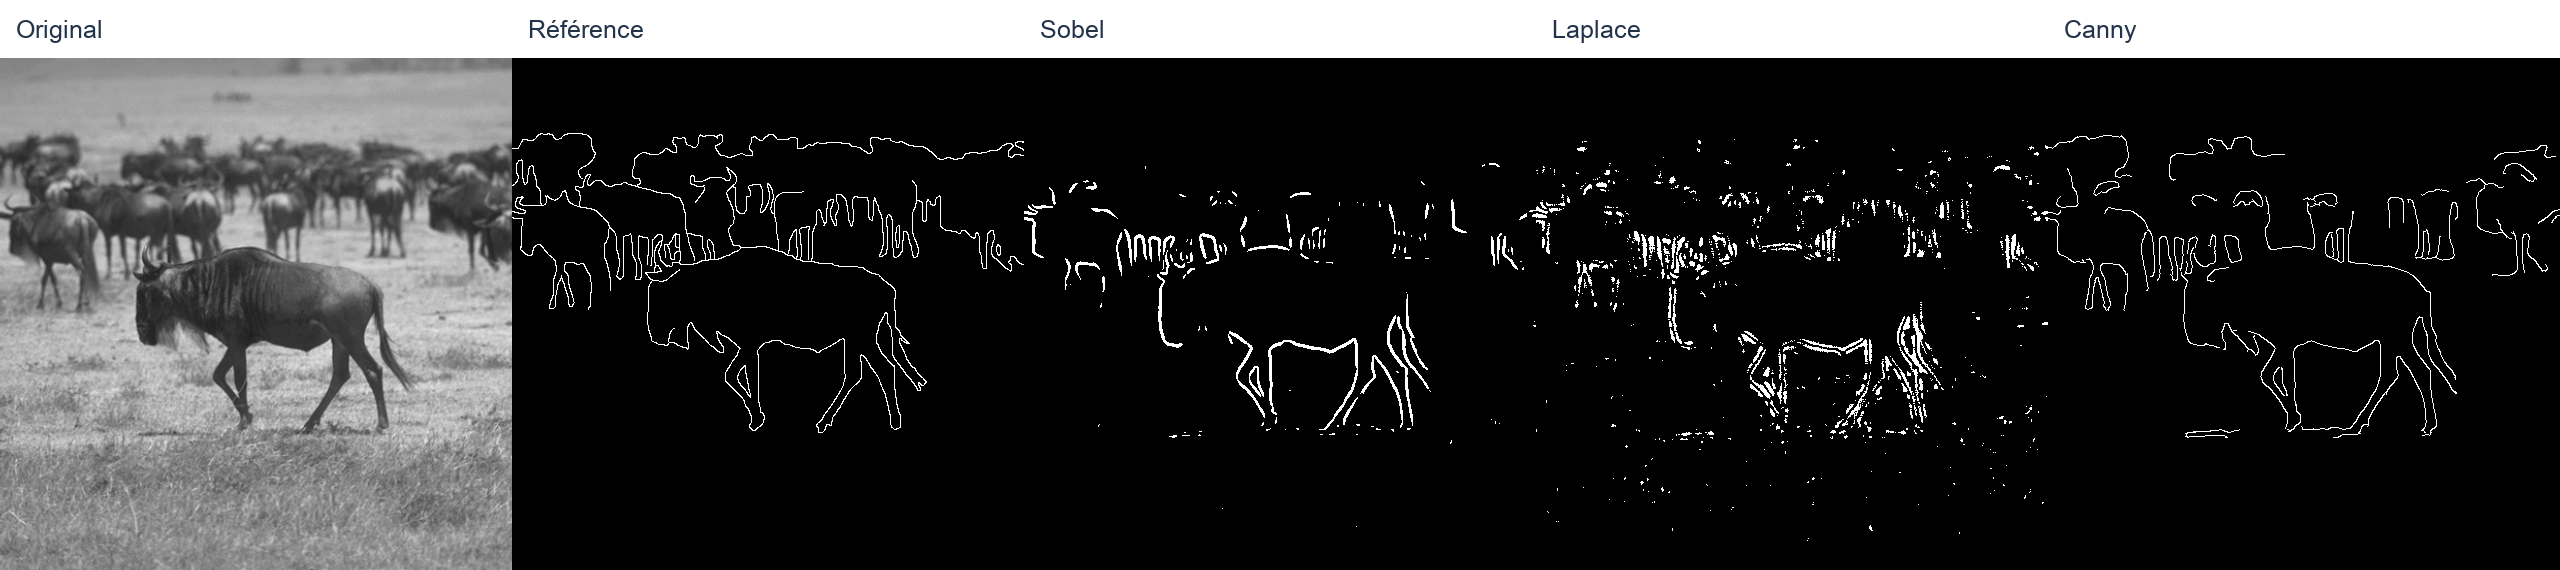
\includegraphics[width=\linewidth]{gnu_comparison.png}
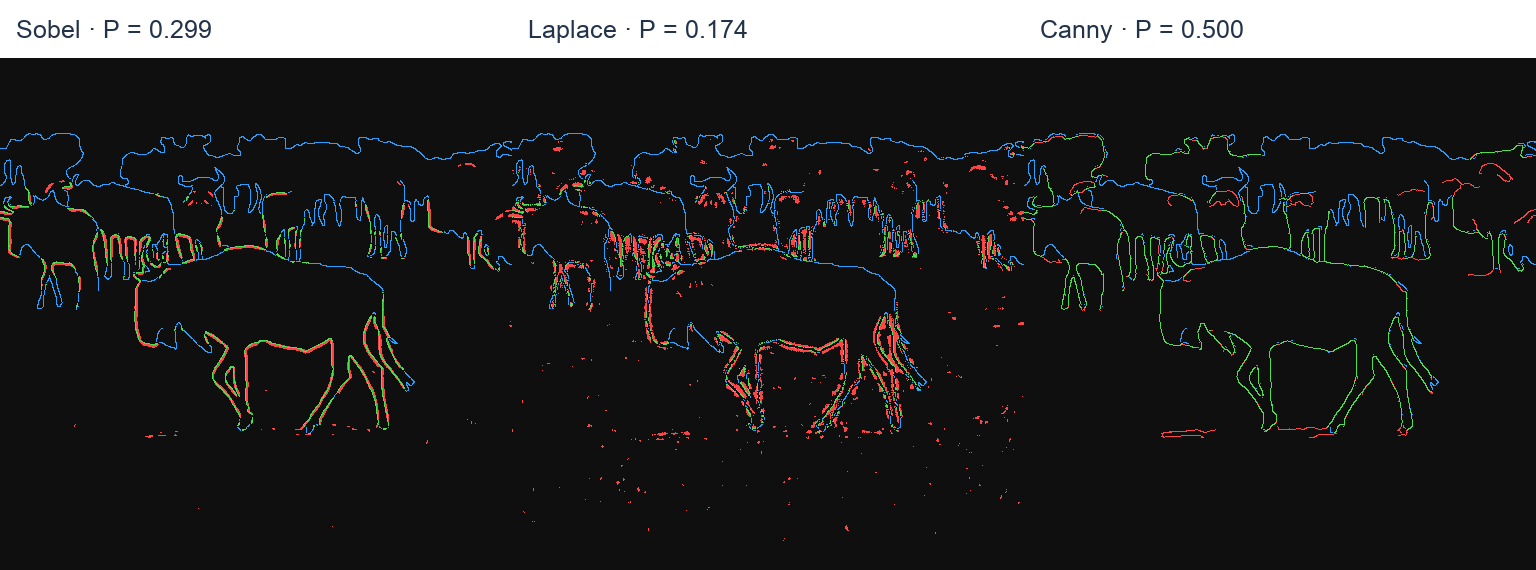
\includegraphics[width=.83\linewidth]{gnu_errors.png}
\captionof{figure}{Image \texttt{gnu} : original, référence et trois détecteurs ; puis superpositions. Vert : correct ; rouge : faux positif ; bleu : faux négatif.}
\end{center}
Sur \api{gnu}, les scores atteignent $0{,}299$ pour Sobel, $0{,}174$ pour Laplace et $0{,}500$ pour Canny. Ce dernier conserve une grande partie des limites de l'animal au premier plan, avec moins de réponses superflues.

\begin{center}
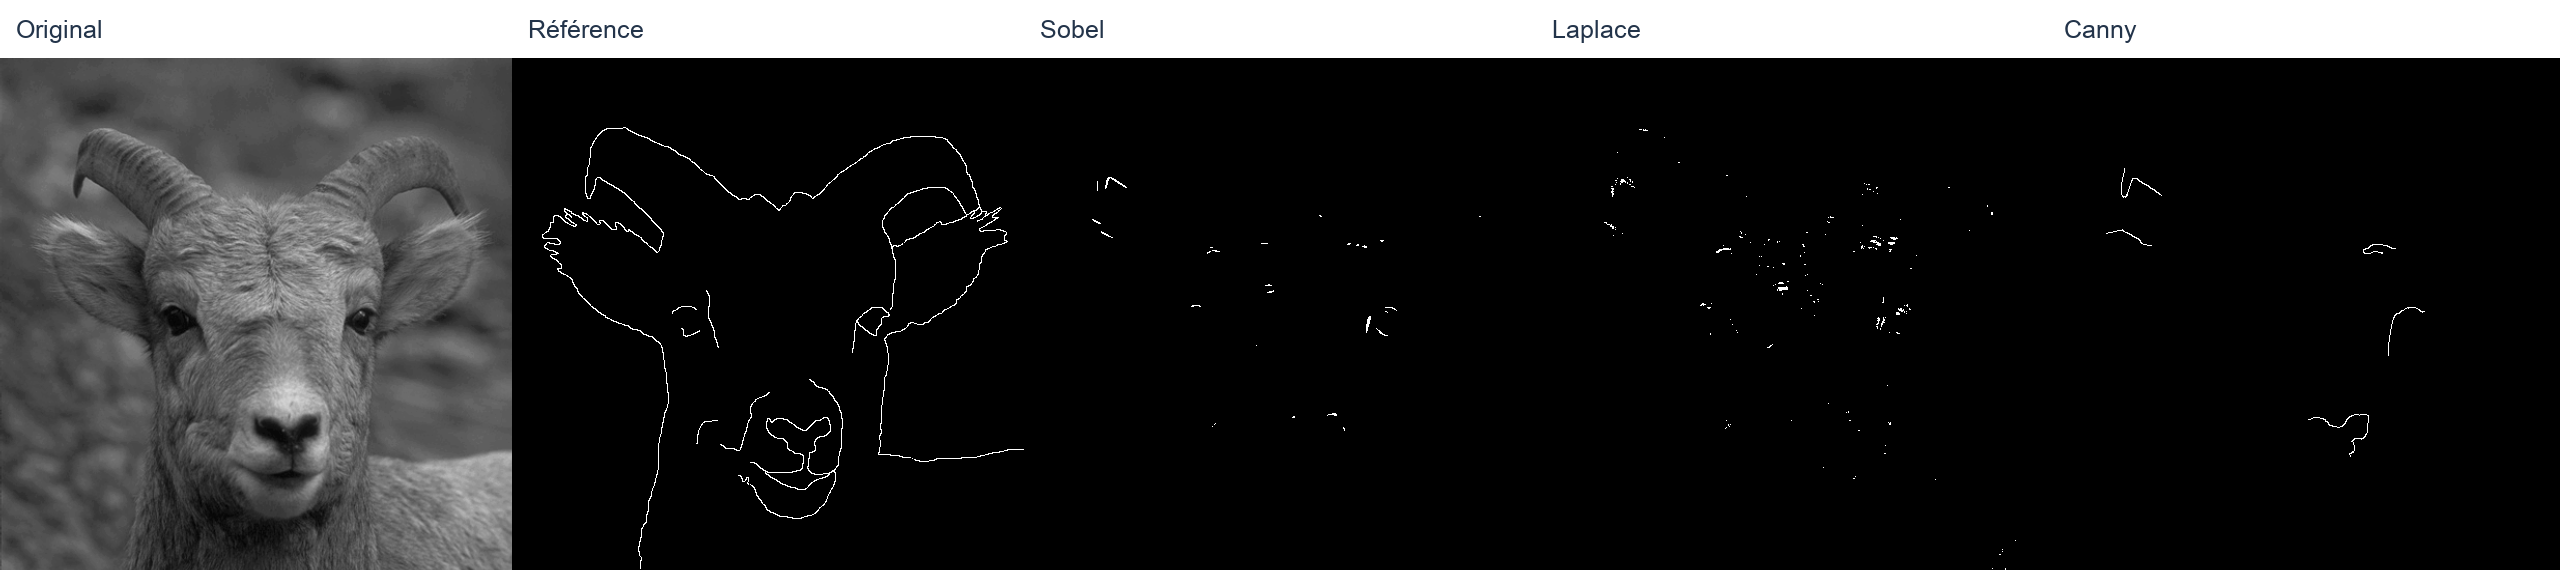
\includegraphics[width=\linewidth]{goat_5_comparison.png}
\captionof{figure}{Image \texttt{goat\_5} : les paramètres globaux manquent une grande partie du contour annoté.}
\end{center}
À l'inverse, sur \api{goat\_5}, les scores sont seulement $0{,}035$, $0{,}017$ et $0{,}057$. Une bonne moyenne ne garantit donc pas une bonne détection sur chaque scène. La cible humaine peut inclure des limites peu contrastées que les dérivées locales révèlent mal.

\clearpage
\section{Influence des paramètres et limites}
\begin{center}
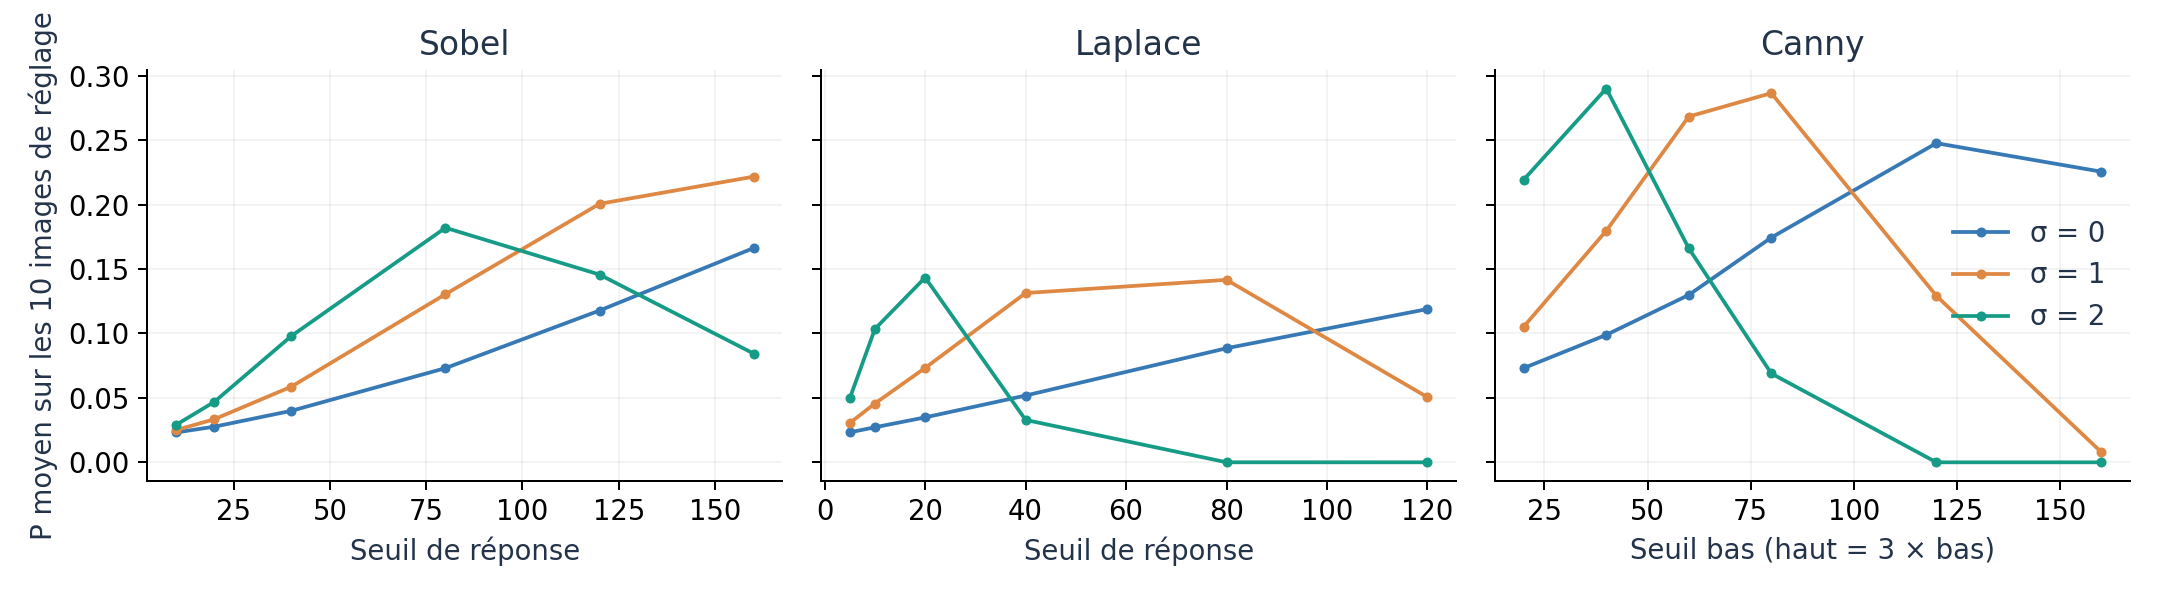
\includegraphics[width=.86\linewidth]{sensitivity.png}
\captionof{figure}{Sensibilité sur les dix images de réglage. Pour Canny, la figure montre le seuil haut égal à trois fois le seuil bas.}
\end{center}
Un seuil faible conserve des détails mais augmente les faux positifs, notamment dans les textures. Un seuil élevé supprime ces réponses et peut manquer de vrais contours. Le lissage réduit les oscillations, tout en modifiant la localisation et l'intensité des dérivées. Les valeurs numériques des seuils ne sont donc pas directement comparables entre détecteurs.

Pour Sobel, le meilleur seuil testé ($T=160$) est en bordure de grille : une recherche élargie pourrait améliorer le résultat. Les noyaux 5 et 7 sont disponibles dans l'interface, mais le protocole garde $k=3$. La séparation 10/30 est unique et certaines familles de scènes apparaissent dans les deux groupes : elle ne démontre pas une généralisation à d'autres types d'images.

La tolérance $3\times3$ absorbe les petits décalages, mais peut aussi accepter une texture voisine. L'appariement maximise le nombre de couples sans minimiser leur distance. La mesure ignore la continuité et le sens des contours. Enfin, une seule annotation humaine est disponible par image : une variation réelle non annotée est comptée comme faux positif.

\section{Utilisation et vérification}
Après compilation avec \api{bash build.sh}, \api{./build/contours -{}-gui} ouvre l'interface à curseurs. La touche \api{s} sauvegarde l'image et ses mesures, \api{b} traite le lot, \api{n/p} change d'image et \api{q} quitte.

Exemple de traitement automatique avec les paramètres de Canny :
\begin{quote}\small\ttfamily
./build/contours -{}-batch -{}-detector canny -{}-sigma 2\\
\hspace*{1em}-{}-low 40 -{}-high 120 -{}-save-images -{}-output results/canny
\end{quote}
Les mesures complètes sont dans \api{results/all\_metrics.csv} : 40 images, trois détecteurs et deux tolérances, soit 240 lignes. \api{scripts/run\_experiments.py} reproduit le protocole. La vidéo commentée est transmise séparément avec le courriel de remise.

Les tests ont réussi sur macOS avec OpenCV 5.0.0 : cartes vides, décalages, double comptage et détecteurs. L'appariement a été comparé à une recherche exhaustive sur 150 petits graphes ; les CSV, les images et les curseurs ont également été contrôlés automatiquement.

\section{Conclusion}
\textbf{Canny est le meilleur compromis moyen avec une tolérance d'un pixel dans ce protocole.} Sobel produit des contours plus épais ; le module du Laplacien est ici moins adapté aux tracés fins. Ce classement dépend des paramètres, de la scène et de la règle de comparaison.

\begingroup\footnotesize
\renewcommand{\refname}{Références}
\begin{thebibliography}{9}\setlength{\itemsep}{0pt}\setlength{\parskip}{0pt}
\bibitem{groningen} C. Grigorescu, N. Petkov et M. A. Westenberg. \emph{Contour detection based on non-classical receptive field inhibition}, IEEE TIP, 12(7), 729--739, 2003. \href{https://www.cs.rug.nl/~imaging/databases/contour_database/contour_database.html}{Base de Groningen}.
\bibitem{sobel} OpenCV. \href{https://docs.opencv.org/4.x/d2/d2c/tutorial_sobel_derivatives.html}{Sobel Derivatives}.
\bibitem{laplace} OpenCV. \href{https://docs.opencv.org/4.x/d5/db5/tutorial_laplace_operator.html}{Laplace Operator}.
\bibitem{canny} OpenCV. \href{https://docs.opencv.org/4.x/da/d22/tutorial_py_canny.html}{Canny Edge Detection}.
\end{thebibliography}
\endgroup
\end{document}
